\section{Example Applications}
\label{sec:example_applications}

\subsection{Line Network Example}

\subsubsection{Traffic Factor}
First, we can provide an example of developing a distribution for $TF_i$ for a line network.

Let's examine an arbitrary flow from source node $i$ and destination as $j$.  We will construct a distribution for $TF_i$ assuming that $i < \frac{N}{2}$.  Since the network is symmetrical, the derivation holds for all nodes.  For a node $x$ in the network, the probability that the flow from $i$ to $j$ goes through $x$ is $\frac{2(x-1)(N-x)}{N(N-1)}$.  Considering the network has $N$ concurrent flows, the number of expected paths going through $x$, then, is: %the number of nodes on one side, $i-1$, multiplied by the number of nodes on the oppposited side, $N-i$:
\begin{equation*}
	\rho(x) = \frac{2(x-1)(N-x)}{N-1}
\end{equation*}

$x$ is a binomial variable with $n = 2(x-1)(N-x)$ and $p = \frac{1}{N-1}$, so it can be approximated with a Gaussian with mean $\frac{2(x-1)(N-x)}{N-1}$ and variance $\frac{2(x-1)(N-x)}{N-1}(1-\frac{1}{N-1})$ (or maybe $\frac{1}{N}$?)

It is easy to show that $\rho(x)$ is increasing in the domain $[1,N/2)$ with the maximum at $N/2$.  Therefore, the value of $x'$ is given by: 

\begin{eqnarray*}
	x' &=&
		\left\{\begin{array}{ll}
		i & \mbox{    } j < i \\
		j & \mbox{    } i < j < \frac{N}{2} \\
		\frac{N}{2} & \mbox{    } \frac{N}{2} \leq j \leq N \\ 
		0 &\mbox{o.w.}
		\end{array}\right.
\end{eqnarray*}

Assuming that all values of $j$ are equally likely, which holds since $p_f$ is equal for all flows, the probability distribution of $x'$ for a flow originating in node $i$ would be

\begin{eqnarray}
	f_{X_i'}(x') &=&
		\left\{\begin{array}{ll}
		\frac{i}{N} & x' = i  \\
		 \frac{1}{2} - \frac{i}{N} & i < x' < \frac{N}{2} \\
		 \frac{1}{2} & x' = \frac{N}{2} \\ 
		0 &\mbox{o.w.}
		\end{array}\right.
		\label{eq:PDF_x_prime}
\end{eqnarray}

Then, the distribution of the PDF for the Traffic Factor of a flow originating in node $i$ is given by Equation (\ref{eq:pdf_TF_1}), where $x'$ is first sampled from the distribution in Equation (\ref{eq:PDF_x_prime}).  This distribution can be fully described with a mixture distribution as follows:

\begin{eqnarray}
\nonumber
	f_{TF}^i (tf) = &&\frac{i}{N} \cdot \mathcal{N}( \rho(i) p_f, \sqrt{\rho(i) p_f (1-p_f)} )  \\ \nonumber
			   &+& \sum\limits_{k=i}^{\frac{N}{2}-1} \cdot \frac{\frac{1}{2}-\frac{i}{N}}{\frac{N}{2} - i}\mathcal{N}( \rho(k) p_f, \sqrt{\rho(k) p_f (1-p_f)} )  \\
			   &+& \frac{1}{2} \cdot \mathcal{N} ( \rho({\frac{N}{2}}) p_f, \sqrt{\rho(\frac{N}{2}) p_f (1-p_f)} )
\label{eq:full_PDF_TF}
\end{eqnarray}

If the expected traffic is for each node to be the source of $1$ flow at a time, on average, then we can substitute a value of $p_f = 1/(N-1)$:

%\begin{eqnarray}
%\nonumber
%	f_{TF}^i (tf) = &&\frac{i}{N} \cdot \mathcal{N}( \frac{\rho_i}{N-1} , \frac{\rho_i  (1-\frac{1}{N-1})}{N-1} )  \\ \nonumber
%			   &+& \sum\limits_{k=i}^{\frac{N}{2}-1} \cdot \frac{\frac{1}{2}-\frac{i}{N}}{\frac{N}{2} - i}\mathcal{N}( \frac{\rho_k}{N-1}, \frac{\rho_k}{N-1} (1-\frac{1}{N-1}) )  \\
%			   &+& \frac{1}{2} \cdot \mathcal{N} ( \frac{\rho_{\frac{N}{2}}}{N-1} , \frac{\rho_{\frac{N}{2}}}{N-1} (1-\frac{1}{N-1}) )
%\label{eq:full_PDF_TF_line}
%\end{eqnarray}

\begin{figure*}
\begin{eqnarray}
\nonumber
	f_{TF}^i (tf) = &&\frac{i}{N} \cdot \mathcal{N}( \frac{2(i-1)(N-i)}{(N-2)(N-1)} , \sqrt{\frac{2(i-1)(N-i)  (1-\frac{1}{N-1})}{(N-2)(N-1)}} )  \\ \nonumber
			   &+& \sum\limits_{k=i}^{\frac{N}{2}-1} \cdot \frac{\frac{1}{2}-\frac{i}{N}}{\frac{N}{2} - i}\mathcal{N}( \frac{2(k-1)(N-k)}{(N-2)(N-1)}, \sqrt{\frac{2(k-1)(N-k)}{(N-2)(N-1)} (1-\frac{1}{N-1})} )  \\
			   &+& \frac{1}{2} \cdot \mathcal{N} ( \frac{N(\frac{N}{2}-1)}{(N-2)(N-1)} , \sqrt{\frac{N(\frac{N}{2}-1)}{(N-2)(N-1)} (1-\frac{1}{N-1})} )
\label{eq:full_PDF_TF_line_2}
\end{eqnarray}
\end{figure*}

\begin{figure}
\begin{centering}
    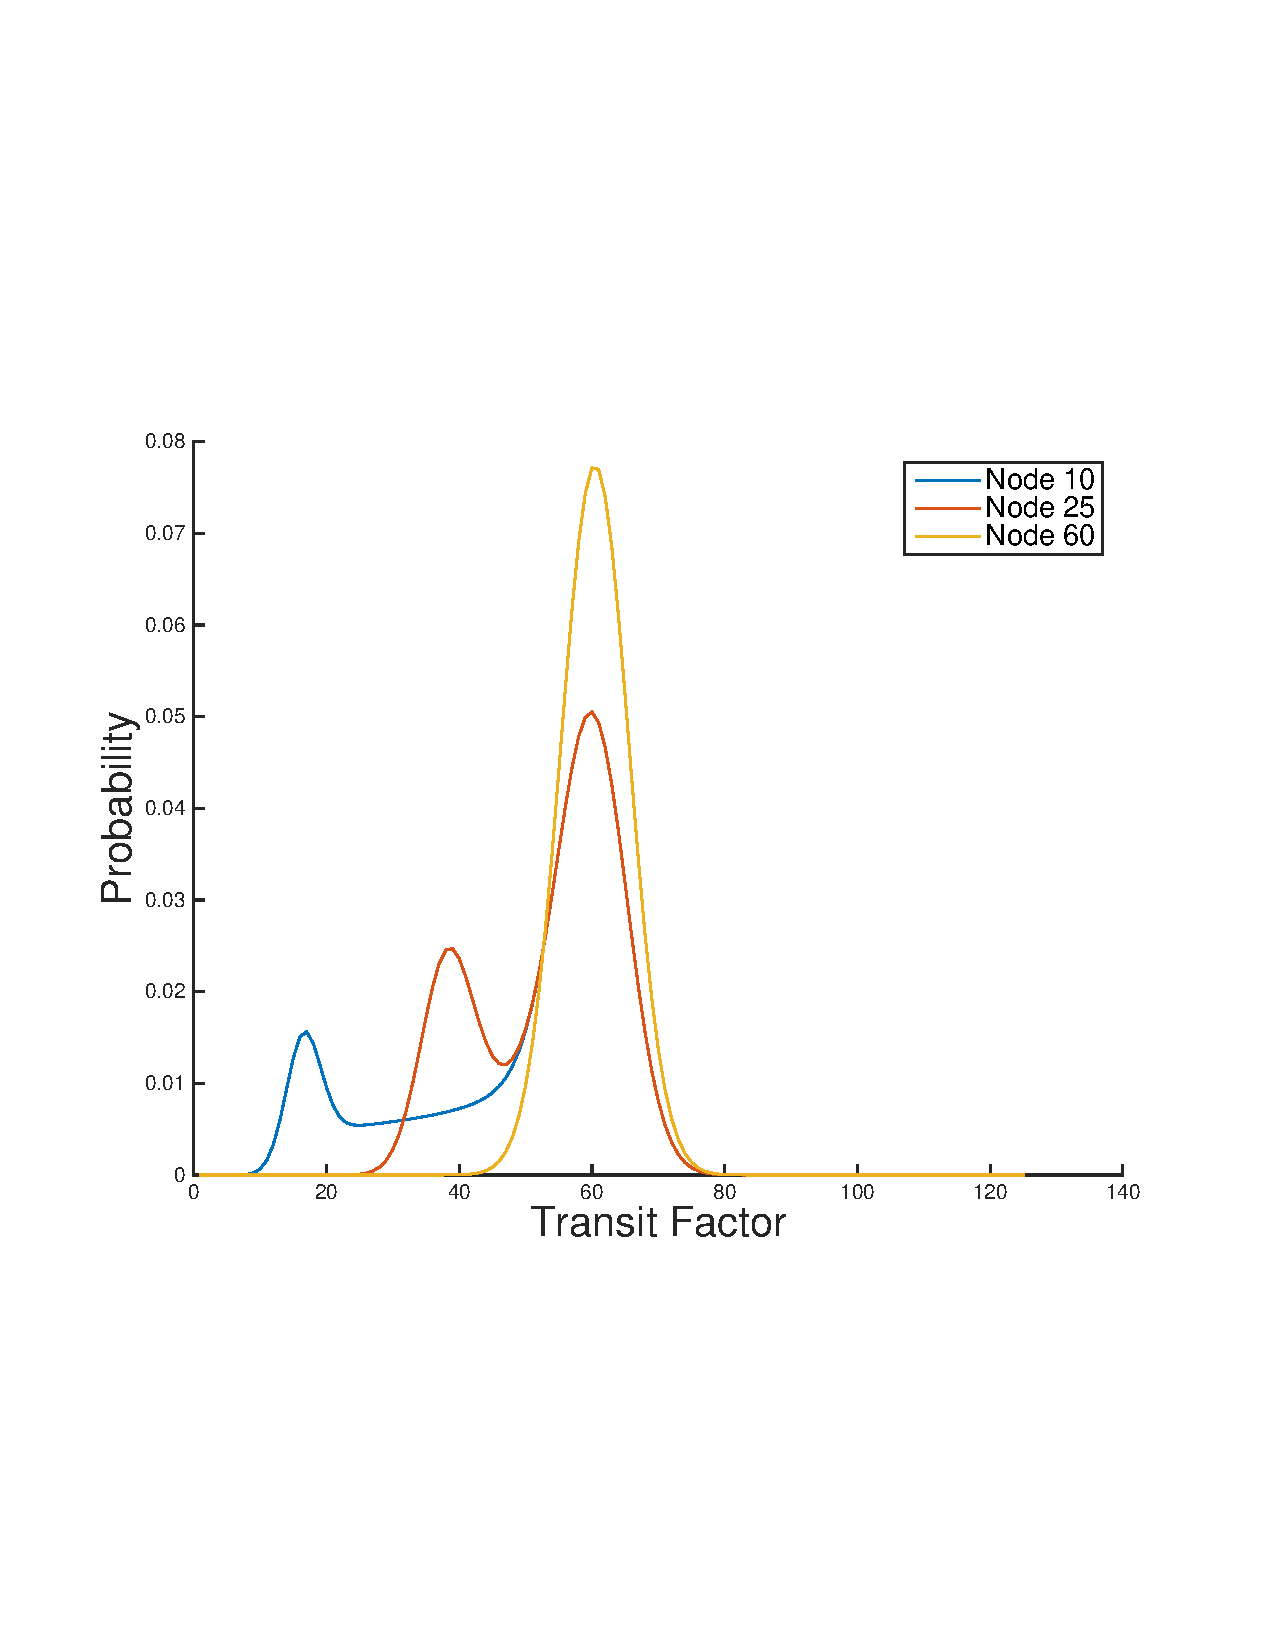
\includegraphics[scale=0.4, clip=true, trim=15mm 65mm 20mm 65mm]{figures/PDF_TF_line_net_125.pdf}
    \caption{PDF of Traffic Factor for flows originating in several different nodes in a 125 node line network.}
    \label{fig:PDF_TF_line_net}
\end{centering}
\end{figure}

\begin{figure}
\begin{centering}
    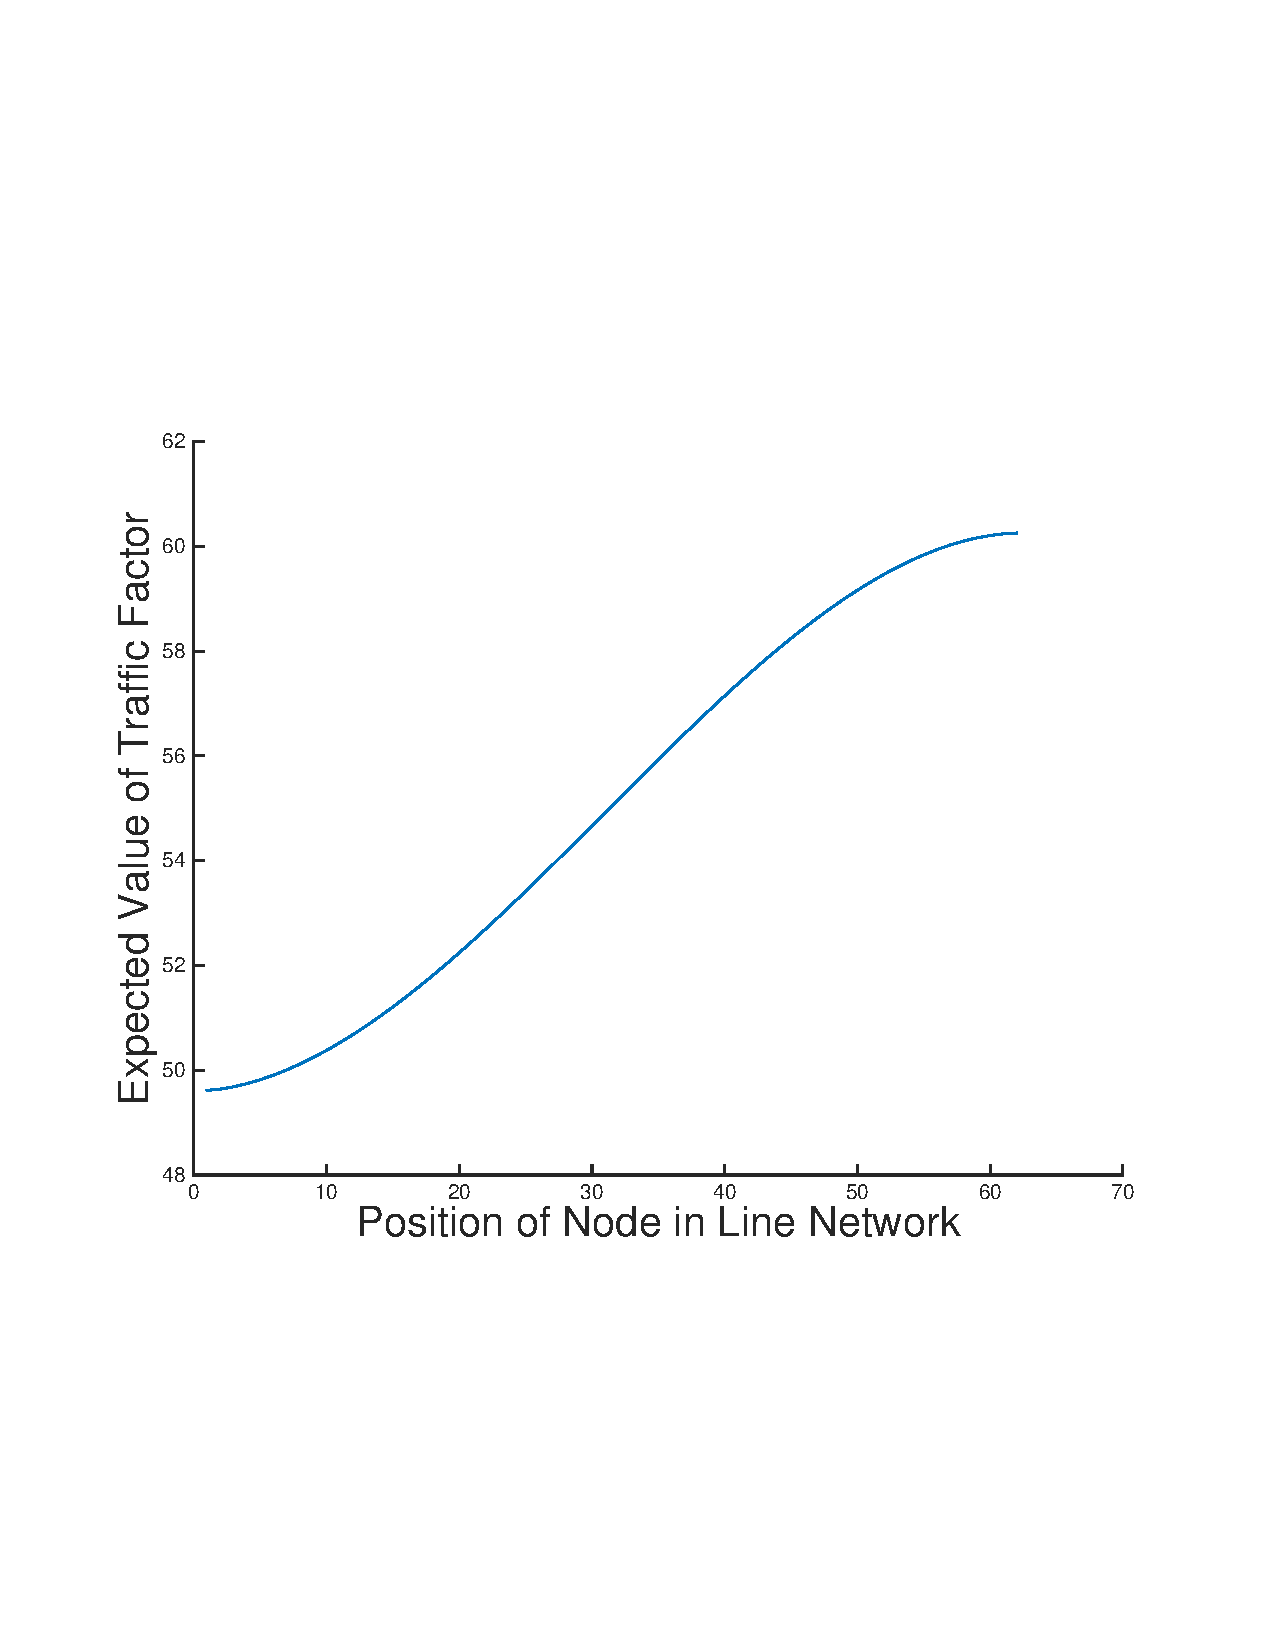
\includegraphics[scale=0.4, clip=true, trim=15mm 65mm 20mm 65mm]{figures/EV_TF_line_net_125.pdf}
    \caption{The expected value of the Traffic Factor is naturally highest in the middle of the line network where more congestion exists.}
    \label{fig:EV_TF_line_net}
\end{centering}
\end{figure}

Figure \ref{fig:PDF_TF_line_net} shows the distribution in Equation \ref{eq:full_PDF_TF} for several chosen nodes in a line network.  Figure \ref{fig:EV_TF_line_net} displays the expected value of TF for flows originating in nodes $1$ to $62$ in a $125$ node line network.  

\subsubsection{Path Length}

%\begin{figure}
%\begin{centering}
%    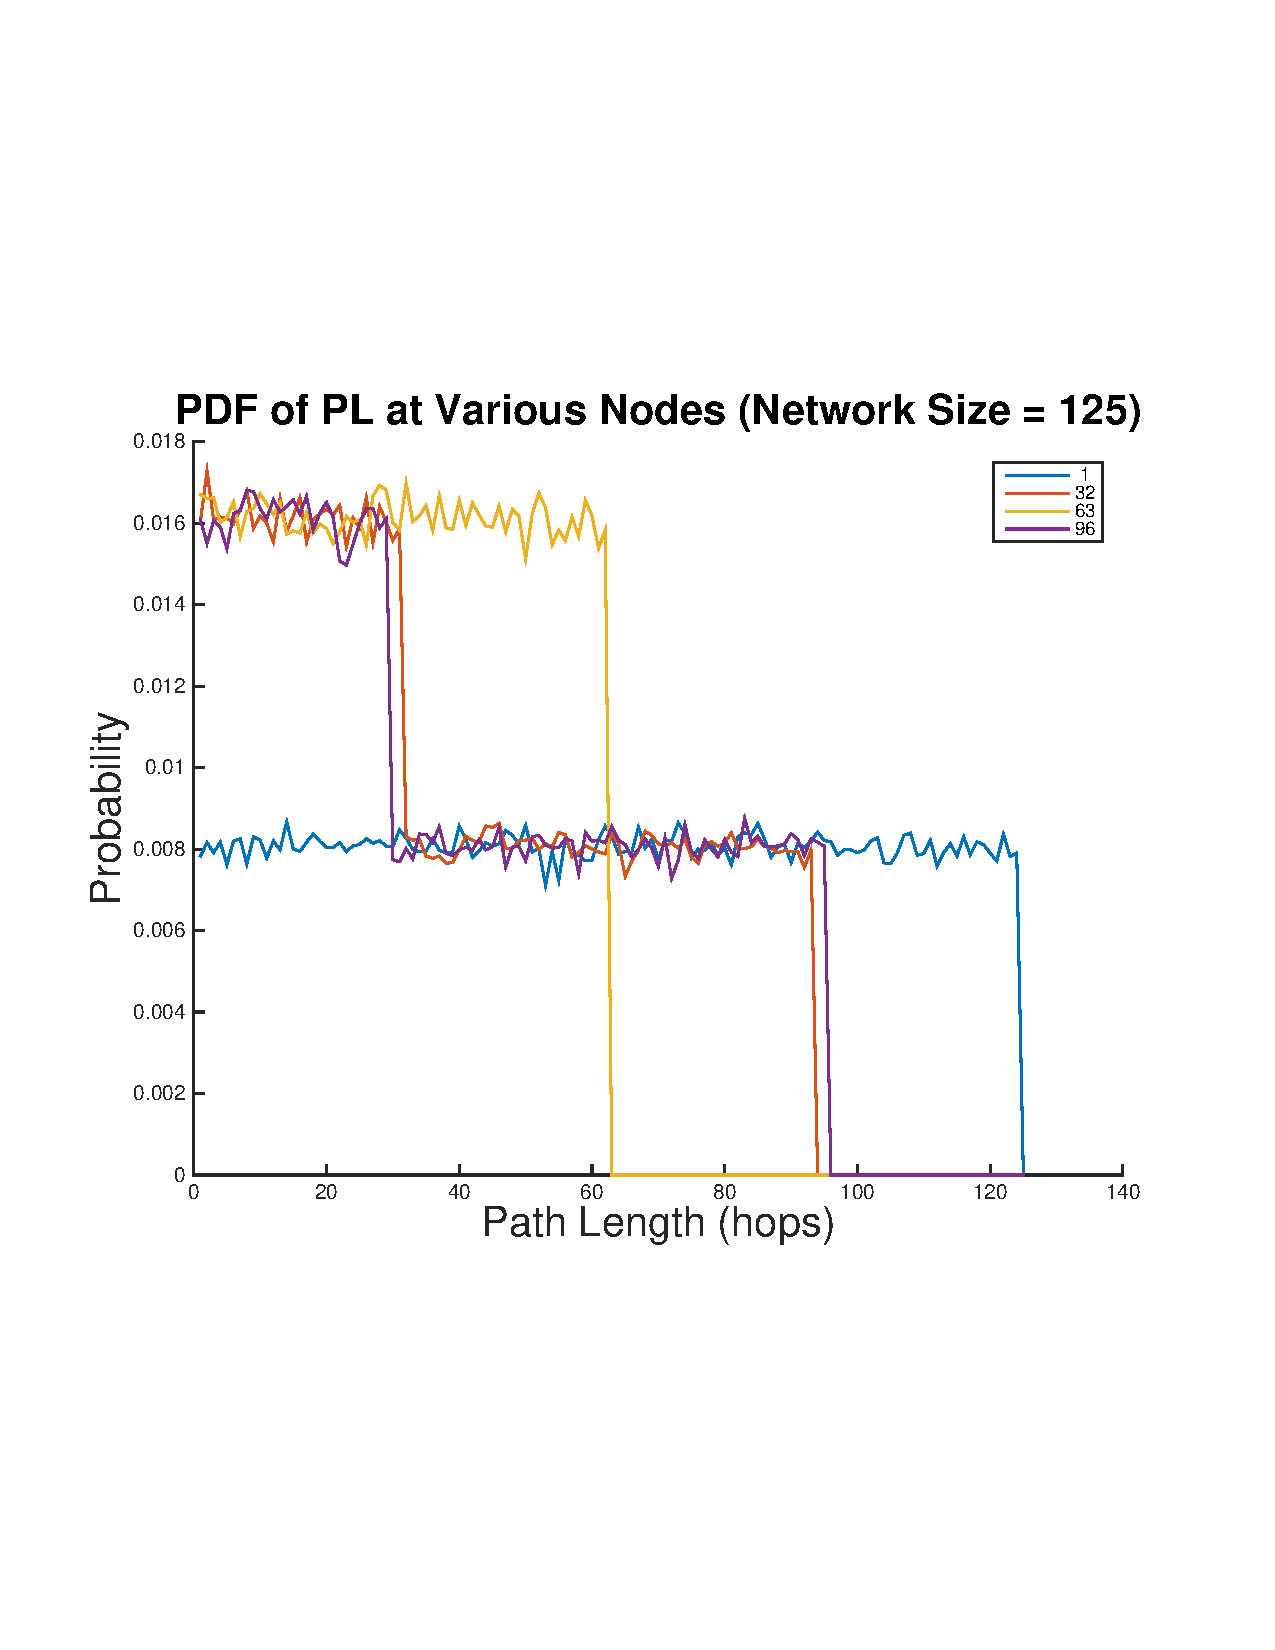
\includegraphics[scale=0.4, clip=true, trim=15mm 65mm 20mm 65mm]{figures/PL_PDFs_each_node_line_net_125.pdf}
%    \caption{Plotting the frequency of experienced Path Lengths for different node positions in a line network shows that PL can be modeled as disjoint Uniform Random Variables.}
%    \label{fig:PL_PDFs_line_net}
%\end{centering}
%\end{figure}
\begin{figure}
\begin{centering}
    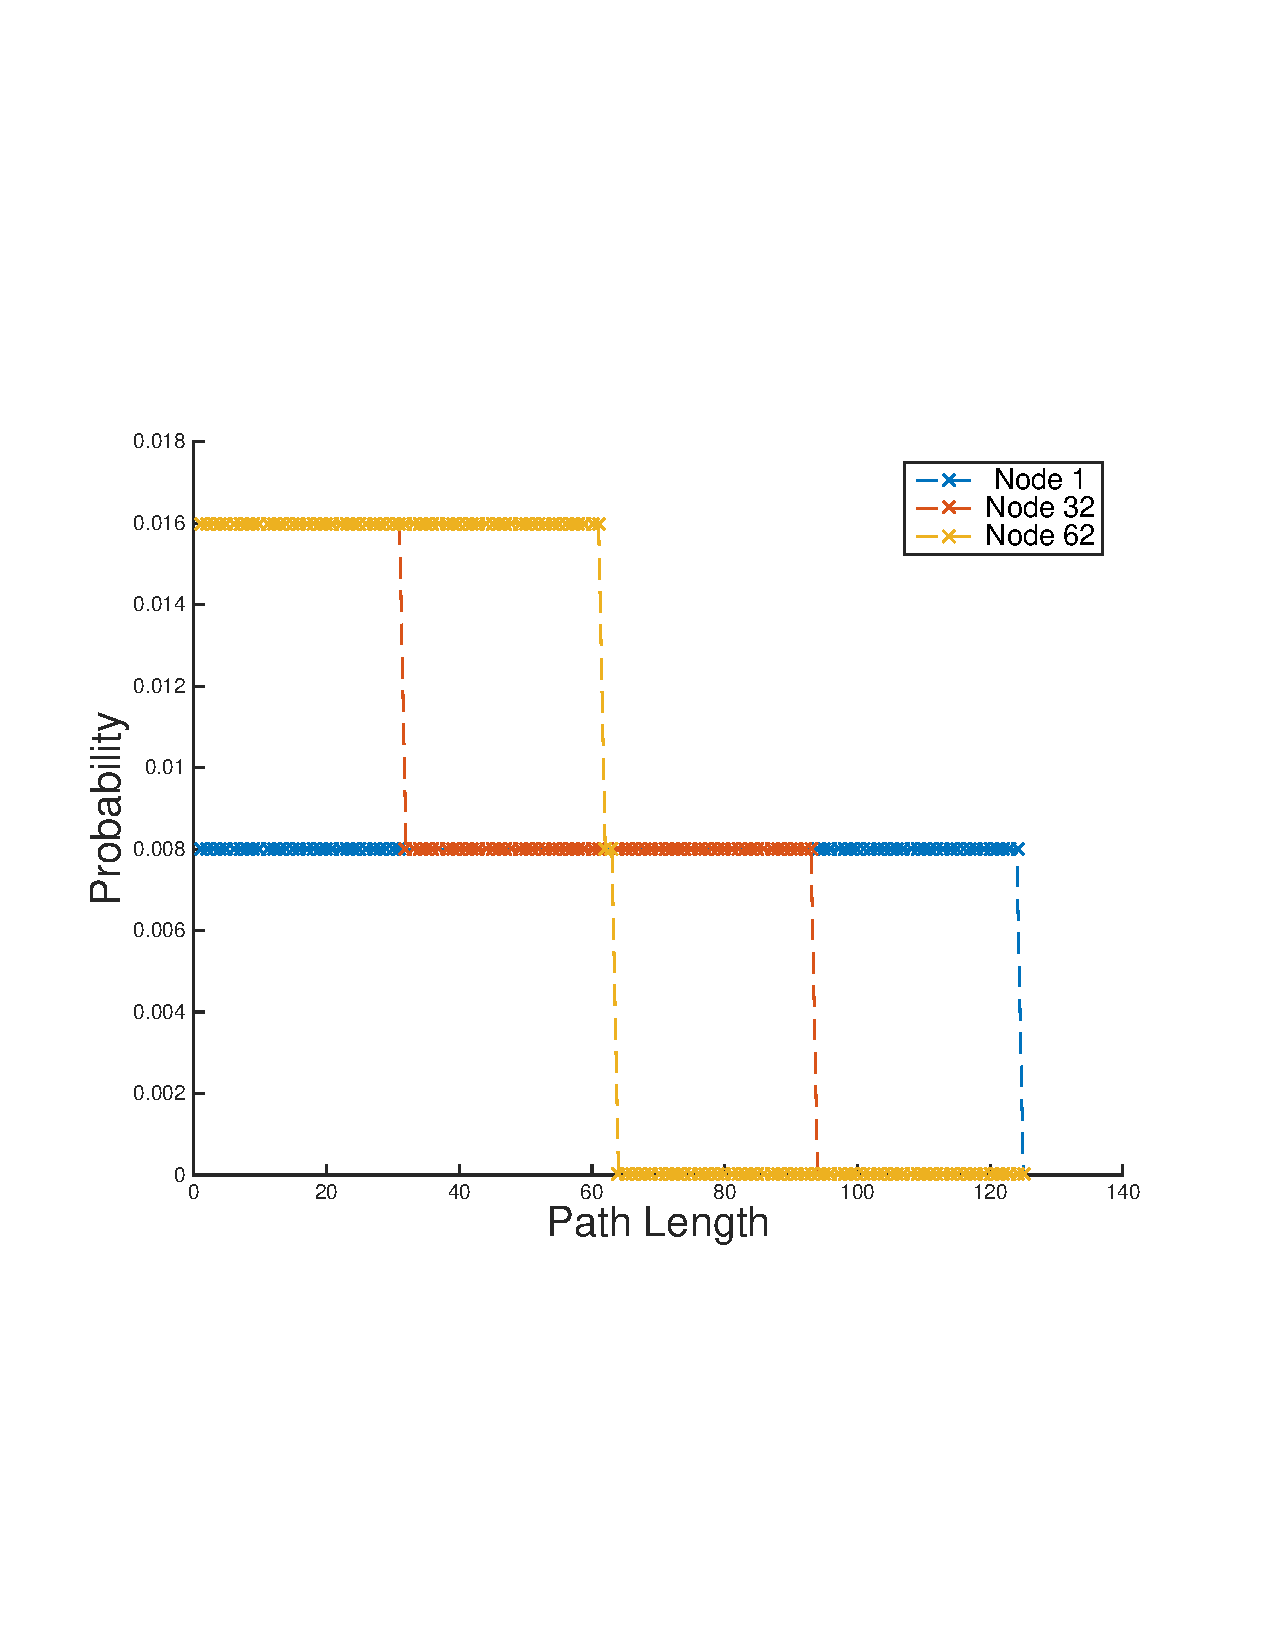
\includegraphics[scale=0.4, clip=true, trim=15mm 65mm 20mm 65mm]{figures/PDF_PL_line_net_125.pdf}
    \caption{PDF of Path Lengths for flows originating in edge cases of a line network.}
    \label{fig:PL_PDFs_line_net}
\end{centering}
\end{figure}

Next, we can capture the distribution of the path length given by flows originating in node $i$ of a line network.

Since our traffic model is to choose destination nodes with uniform randomness, we can derive the distribution of path lengths for flows with source node $i$ as follows (details can be given if needed).  Again, let us just assume that $i$ is less than $N/2$, since we can use symmetry to draw the same conclusion about nodes greater than $N/2$.  The following is the distribution, which is shown in Figure \ref{fig:PL_PDFs_line_net} for the edge cases of $i=1$ and $i=63$, the nodes on the end and in the middle of the line network, respectively. 

\begin{eqnarray}
	f_{PL_i}(pl) &=&
		\left\{\begin{array}{ll}
		\frac{2}{N} & \mbox{for } 1 \leq pl \leq i-1 \\
		\frac{1}{N} & \mbox{for } i \leq pl \leq N-i \\
		0 &\mbox{elsewhere}
		\end{array}\right.
\label{eq:full_PDF_PL}
\end{eqnarray}

\begin{figure}
\begin{centering}
    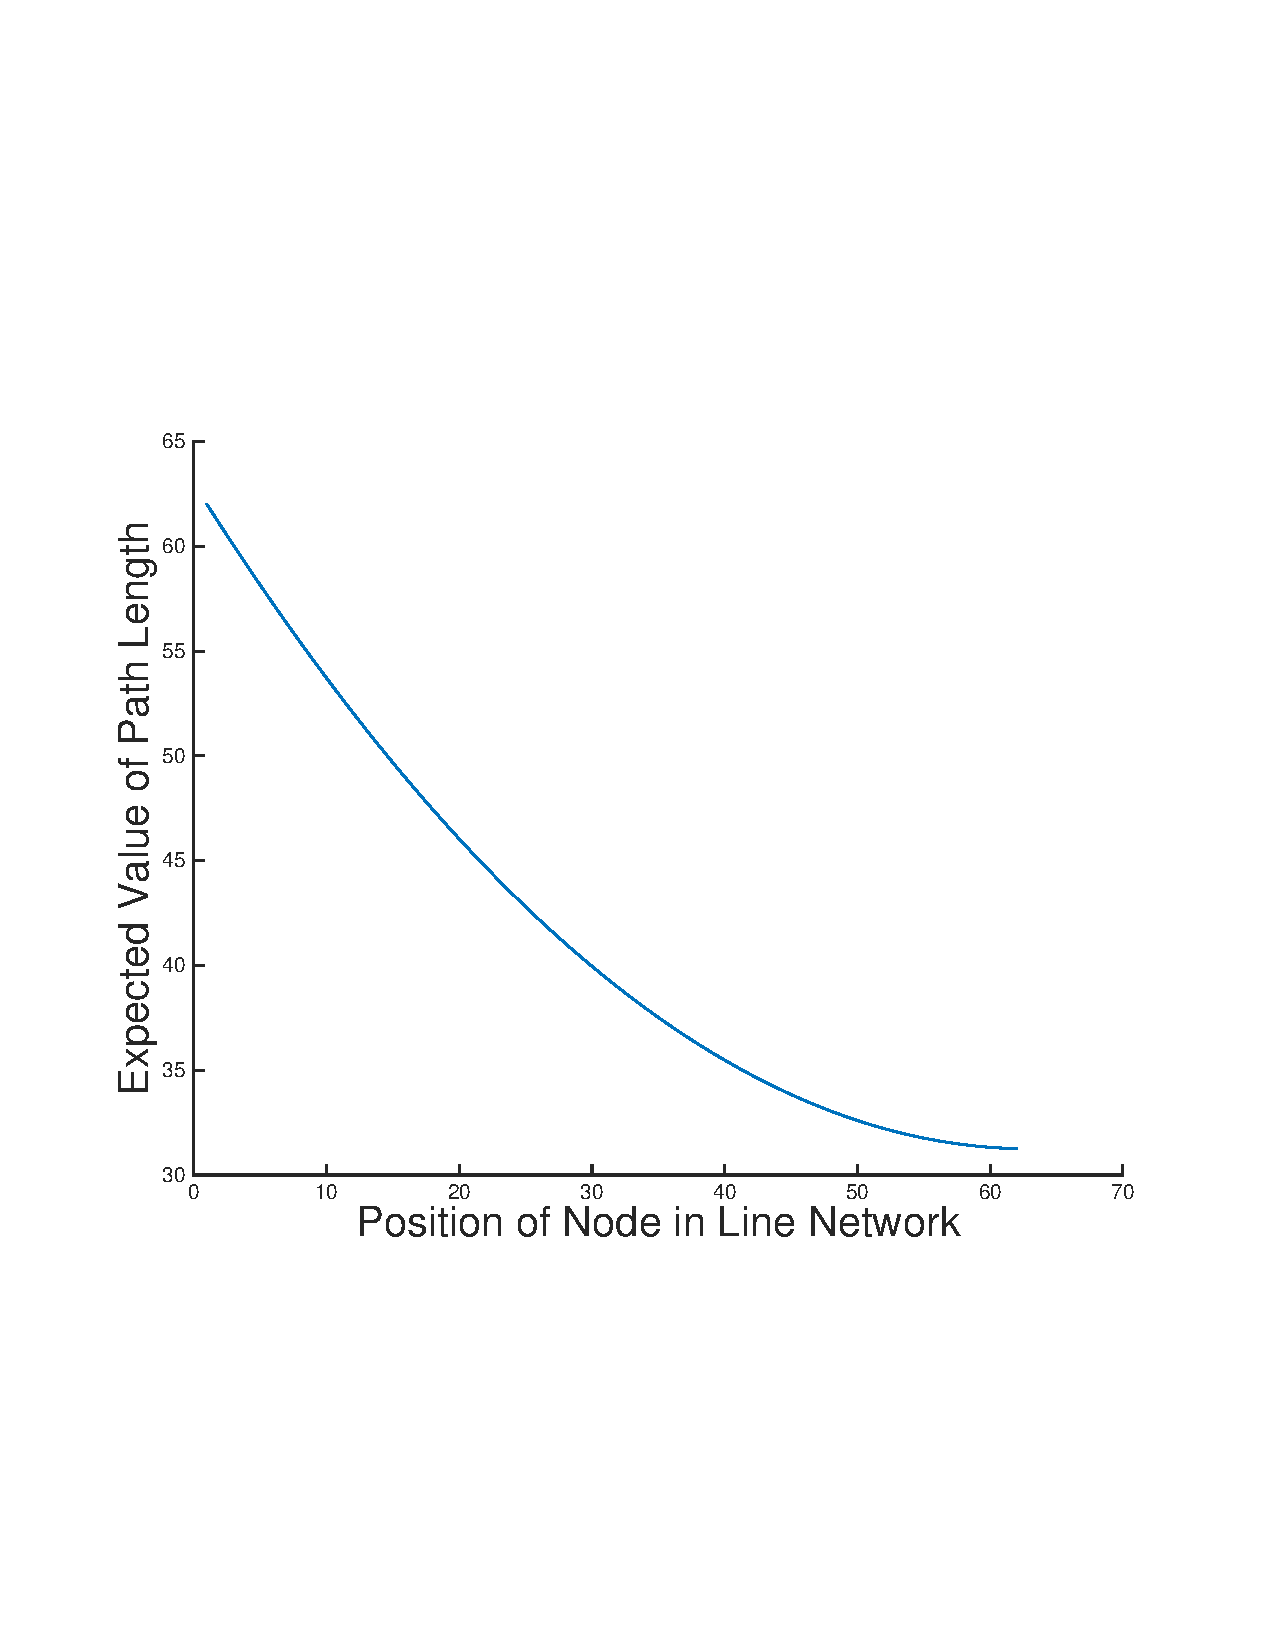
\includegraphics[scale=0.4, clip=true, trim=15mm 65mm 20mm 65mm]{figures/EV_PL_line_net_125.pdf}
    \caption{The expected value of path length intuitively peaks at the edges of the line network and is minimum in the middle.}
    \label{fig:mean_PL_each_node_line_net}
\end{centering}
\end{figure}

From (\ref{eq:full_PDF_PL}), we can derive the following expression for the expected value of a path length for a flow originating in node $i$.

\begin{equation}
	E[PL_i] = \frac{N}{2} + \frac{i^2}{N} - \frac{2 \cdot i}{N} - i
\end{equation}

These expected values for path length of flows originating in different nodes are shown in Figure \ref{fig:mean_PL_each_node_line_net}.  Not surprisingly, values of mean path length range from $~N/2$ at the end of the network to $~N/4$ in the middle of the network.  


%Is the Delay Factor dependent on node position?  It must be...similar to path length, a node's position affects the probability of choosing a route with or against the flow of scheduling.  
%Finally, we can give a simple expression for the Delay Factor: 
%\begin{eqnarray*}
%	P_{DF_x}(l) &=&
%		\left\{\begin{array}{ll}
%		\frac{2}{N} & \mbox{for } 1 < l < \min(i,N-i) \\
%		\frac{1}{N} & \mbox{for } \min(i,N-i) \leq l \leq \max(i,N-i) \\
%		0 &\mbox{elsewhere}
%		\end{array}\right.
%\end{eqnarray*}


